% !TEX program = xelatex
\documentclass[aspectratio=169,10pt]{beamer}

\usepackage[UTF8,noindent]{ctex}
\usepackage{tikz}
\usetikzlibrary{positioning, arrows.meta, fit, backgrounds, calc}
\usepackage{booktabs}
\usepackage{multirow}
\usepackage{graphicx}
\usepackage{amsmath}
\usepackage{array}

% ============================================================
% Tsinghua University Color Theme
% ============================================================
\definecolor{thupurple}{HTML}{660874}
\definecolor{thugold}{HTML}{C49B0C}
\definecolor{thulightpurple}{HTML}{F0E6F6}
\definecolor{thugray}{HTML}{4A4A4A}
\definecolor{thulightgray}{HTML}{F5F5F5}

\usetheme{Madrid}
\usecolortheme[named=thupurple]{structure}
\setbeamercolor{title}{fg=white,bg=thupurple}
\setbeamercolor{frametitle}{fg=white,bg=thupurple}
\setbeamercolor{block title}{fg=white,bg=thupurple}
\setbeamercolor{block body}{bg=thulightpurple}
\setbeamercolor{item}{fg=thupurple}
\setbeamercolor{enumerate item}{fg=thupurple}
\setbeamercolor{section in toc}{fg=thupurple}
\setbeamercolor{footline}{fg=thugray,bg=thulightgray}
\setbeamercolor{page number in head/foot}{fg=thugray}
\setbeamertemplate{navigation symbols}{}
\setbeamertemplate{footline}{%
  \leavevmode\hbox{%
    \begin{beamercolorbox}[wd=.5\paperwidth,ht=2.5ex,dp=1ex,left]{footline}%
      \hspace*{2ex}\insertshortauthor\ —\ \insertshorttitle
    \end{beamercolorbox}%
    \begin{beamercolorbox}[wd=.5\paperwidth,ht=2.5ex,dp=1ex,right]{footline}%
      \insertframenumber/\inserttotalframenumber\hspace*{2ex}
    \end{beamercolorbox}%
  }%
}

\graphicspath{{figures/}}

% ============================================================
% Title Page Information
% ============================================================
\title{基于多模态大语言模型的数字电路时序图解析}
\subtitle{本科毕业论文答辩}
\author{汤秉达}
\institute{清华大学\ 计算机科学与技术系\\[0.3em]
指导教师：喻文健\ 教授}
\date{2026年6月}

\begin{document}

% ============================================================
% Title Page
% ============================================================
{
\setbeamertemplate{footline}{}
\begin{frame}
\vspace{1em}
\begin{columns}
\begin{column}{0.15\textwidth}
\centering
\includegraphics[height=1.8cm]{thu-fig-logo.pdf}
\end{column}
\begin{column}{0.85\textwidth}
\titlepage
\end{column}
\end{columns}
\end{frame}
}

% ============================================================
% Outline
% ============================================================
\begin{frame}{提纲}
\tableofcontents
\end{frame}

% ============================================================
\section{研究背景与动机}
% ============================================================

\begin{frame}{研究背景}
\begin{columns}[T]
\begin{column}{0.55\textwidth}
\textbf{数字电路时序图}是芯片设计中定义模块行为的核心视觉规范：
\begin{itemize}
  \item 编码信号间的先后次序与因果关系
  \item 广泛用于协议规范（SPI、I2C、AXI等）
  \item 是设计者实现HDL代码的权威依据
\end{itemize}

\vspace{0.8em}
\textbf{现状痛点：}
\begin{itemize}
  \item 从时序图到HDL代码\alert{完全依赖手工}
  \item 效率低下：复杂协议需数小时人工解读
  \item 容易出错：细微依赖关系极易被遗漏
\end{itemize}
\end{column}
\begin{column}{0.42\textwidth}
\centering
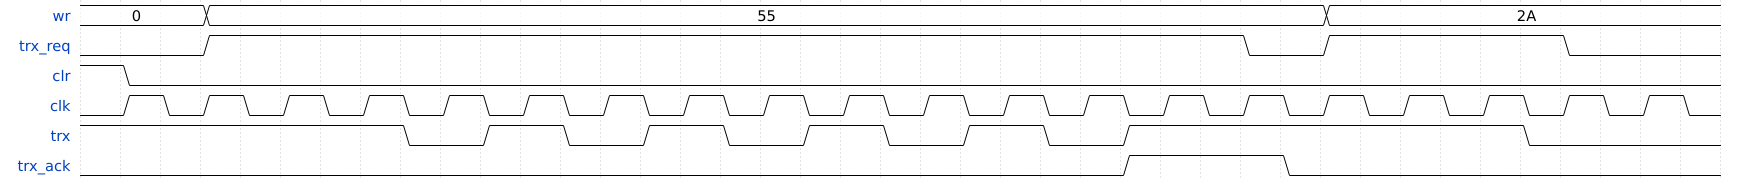
\includegraphics[width=\textwidth]{figures/samples/uart.png}\\[0.3em]
{\footnotesize UART控制器时序图示例}
\end{column}
\end{columns}
\end{frame}

\begin{frame}{技术机遇与挑战}
\textbf{技术机遇：}多模态大语言模型（MLLM）的快速发展
\begin{itemize}
  \item LLM在代码生成任务上已展现强大能力
  \item MLLM具备从视觉输入提取结构化信息的基础能力
\end{itemize}

\vspace{0.5em}
\textbf{核心挑战：}
\begin{enumerate}
  \item \textbf{数据匮乏}——不存在面向时序图解析的高质量标注数据集
  \item \textbf{评价缺失}——传统文本相似度指标（BLEU/ROUGE）无法衡量结构语义正确性
  \item \textbf{领域特化}——时序图视觉特征高度专业化，通用模型零样本效果差
  \item \textbf{功能正确性}——仅靠有监督学习难以保证生成代码的功能行为
\end{enumerate}
\end{frame}

\begin{frame}{已有工作与不足}
\begin{block}{TD-Magic (He et al., 2023)}
基于规则从时序图提取偏序关系，难以扩展到复杂场景
\end{block}

\begin{block}{TD-Interpreter (He et al., 2025)}
对LLaVA微调的视觉问答系统，存在以下局限：
\begin{itemize}
  \item 定位为问答，\alert{不涉及结构化提取与HDL代码生成}
  \item 训练数据采用随机激励，时序图缺乏有意义的功能模式
  \item 评价仅用BLEU/ROUGE，缺乏专用评价方法
  \item 仅SFT训练，未探索强化学习优化
\end{itemize}
\end{block}

\vspace{0.3em}
\centering
$\Longrightarrow$ 本文：\textbf{图像 $\to$ 结构化表示 $\to$ HDL代码}的生成式流水线
\end{frame}

% ============================================================
\section{方法框架}
% ============================================================

\begin{frame}{框架概览}
\centering
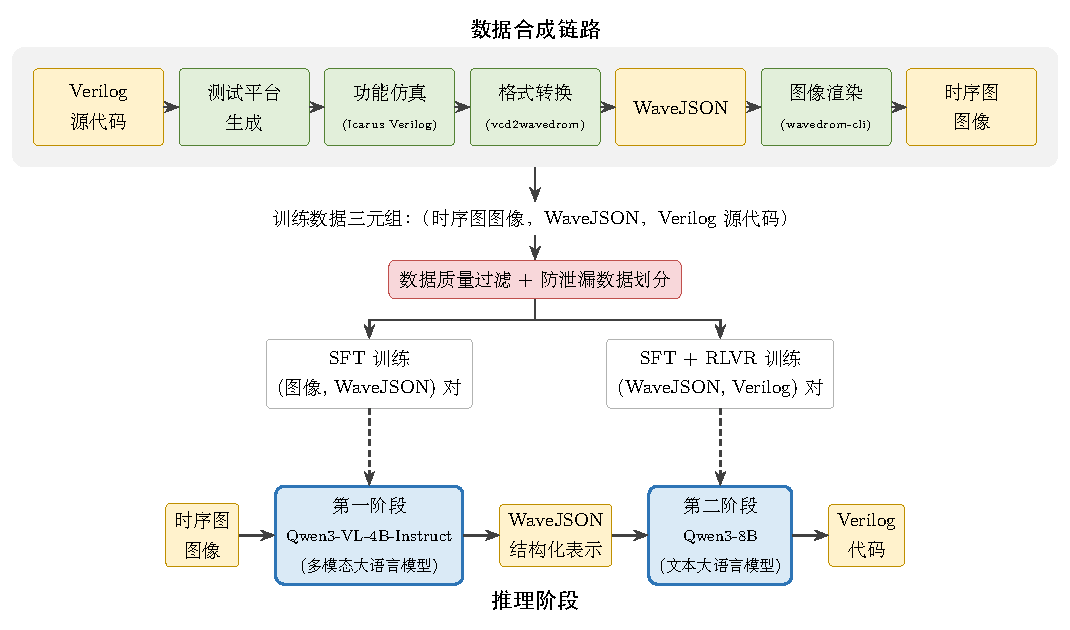
\includegraphics[width=0.92\textwidth]{figures/framework.pdf}
\end{frame}

\begin{frame}{两阶段设计动机}
\begin{columns}[T]
\begin{column}{0.48\textwidth}
\begin{block}{第一阶段：图像 $\to$ WaveJSON}
\begin{itemize}
  \item 模型：Qwen3-VL-4B-Instruct
  \item 核心能力：跨模态视觉理解
  \item 需要多模态感知图像中的信号名、波形、数据标签
\end{itemize}
\end{block}
\end{column}
\begin{column}{0.48\textwidth}
\begin{block}{第二阶段：WaveJSON $\to$ Verilog}
\begin{itemize}
  \item 模型：Qwen3-8B
  \item 核心能力：逻辑推理与代码生成
  \item 从行为描述推断因果逻辑并转化为电路代码
\end{itemize}
\end{block}
\end{column}
\end{columns}

\vspace{1em}
\textbf{解耦的优势：}
\begin{itemize}
  \item 两阶段可独立训练与优化，降低学习难度
  \item 结构化中间表示缩短序列长度，降低显存需求
  \item 各阶段可选用最适合的模型架构
\end{itemize}
\end{frame}

% ============================================================
\section{数据合成与质量保障}
% ============================================================

\begin{frame}{数据合成链路}
从Verilog源代码自动产出训练三元组（图像、WaveJSON、Verilog）：

\vspace{0.5em}
\centering
\begin{tikzpicture}[
  >=Stealth, font=\scriptsize,
  box/.style={draw=thupurple!70, fill=thulightpurple, rounded corners=2pt,
    minimum height=0.7cm, minimum width=1.5cm, align=center, inner sep=2pt},
  arr/.style={->, line width=0.6pt, thugray}
]
\node[box] (v) {Verilog\\源代码};
\node[box, right=0.15cm of v] (qf) {数据质量\\过滤};
\node[box, right=0.15cm of qf] (tb) {测试平台\\生成};
\node[box, right=0.15cm of tb] (sim) {功能仿真};
\node[box, right=0.15cm of sim] (conv) {格式转换};
\node[box, right=0.15cm of conv] (wj) {WaveJSON};
\node[box, right=0.15cm of wj] (render) {图像渲染};
\node[box, right=0.15cm of render] (img) {时序图\\图像};
\draw[arr] (v) -- (qf);
\draw[arr] (qf) -- (tb);
\draw[arr] (tb) -- (sim);
\draw[arr] (sim) -- (conv);
\draw[arr] (conv) -- (wj);
\draw[arr] (wj) -- (render);
\draw[arr] (render) -- (img);
\end{tikzpicture}

\vspace{0.8em}
\begin{columns}[T]
\begin{column}{0.48\textwidth}
\textbf{数据源：}Verilog\_GitHub数据集\\
108,971个文件 $\to$ 筛选后5,847个有效模块
\end{column}
\begin{column}{0.48\textwidth}
\textbf{关键优化点：}
\begin{itemize}
  \item 测试平台生成策略
  \item 多层级数据质量过滤
  \item 防泄漏数据划分
\end{itemize}
\end{column}
\end{columns}
\end{frame}

\begin{frame}{测试平台生成：随机激励 vs LLM激励}
\begin{columns}[T]
\begin{column}{0.48\textwidth}
\textbf{基线：随机激励（gentbvlog）}
\begin{itemize}
  \item 自动生成伪随机输入序列
  \item 优势：完全自动化、适用面广
  \item \alert{局限：缺乏功能语义}
  \item 信号行为退化为常量或噪声
\end{itemize}
\end{column}
\begin{column}{0.48\textwidth}
\textbf{优化：LLM激励（GPT-OSS-120B）}
\begin{itemize}
  \item 分析模块功能后生成针对性激励
  \item 遍历状态机转移路径
  \item 测试计数器边界溢出
  \item 覆盖算术单元典型运算模式
\end{itemize}
\end{column}
\end{columns}

\vspace{0.5em}
\centering
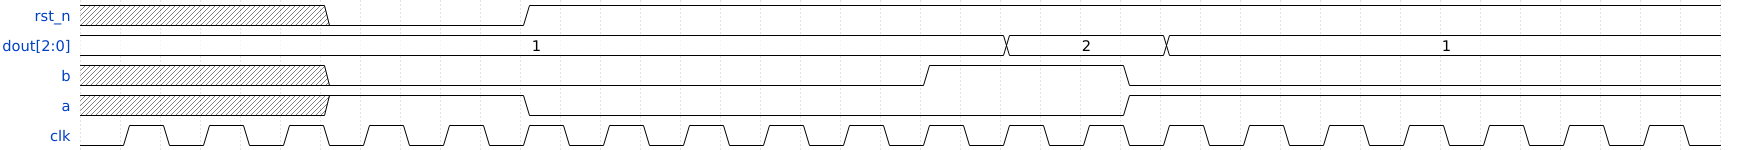
\includegraphics[width=0.46\textwidth]{figures/samples/fsm_new.png}\hfill
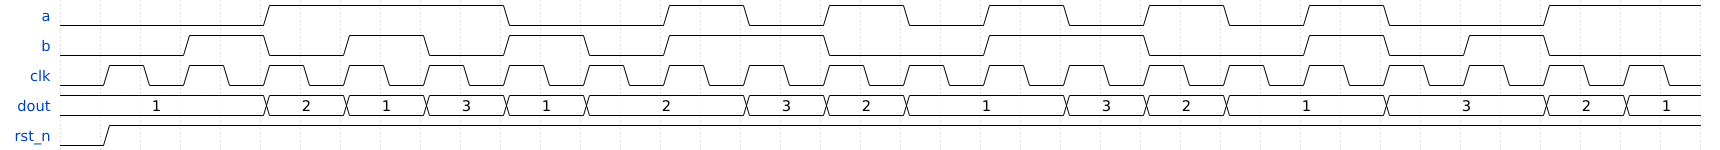
\includegraphics[width=0.46\textwidth]{figures/samples/fsm_new_llm.png}\\
{\footnotesize 左：随机激励（仅触发部分状态）\quad 右：LLM激励（遍历全部状态转移）}
\end{frame}

\begin{frame}{数据质量过滤与防泄漏划分}
\begin{columns}[T]
\begin{column}{0.50\textwidth}
\textbf{多层级质量过滤：}
\begin{enumerate}
  \item \textbf{Verilog源码预筛}
  \begin{itemize}
    \item 排除含\texttt{`include}、\texttt{\$readmemh}的文件
    \item 排除空壳模块、多模块文件
    \item 排除工艺库标准单元
    \item Icarus Verilog语法检查
  \end{itemize}
  \item \textbf{仿真产出质量筛选}
  \begin{itemize}
    \item 图像尺寸与宽高比约束
    \item 信号数量上下界
  \end{itemize}
\end{enumerate}
\end{column}
\begin{column}{0.46\textwidth}
\textbf{防泄漏数据划分：}

基于并查集（DSU）的等价类划分：
\begin{itemize}
  \item WaveJSON指纹匹配
  \item 信号名模糊匹配（阈值0.88）
  \item 同一等价类\alert{整组分配}到同一集合
\end{itemize}

\vspace{0.5em}
\textbf{划分结果：}\\
训练集 5,730 / 测试集 117
\end{column}
\end{columns}
\end{frame}

% ============================================================
\section{评价指标}
% ============================================================

\begin{frame}{专用评价指标设计}
传统文本指标的失效：对语义无关差异过度惩罚，对语义错误不够敏感

\vspace{0.5em}
\textbf{本文指标流程：}
\begin{enumerate}
  \item \textbf{信号匹配}：精确匹配（规范化信号名）+ 模糊匹配（Levenshtein距离，阈值0.7）
  \item \textbf{波形评分}：
  \begin{itemize}
    \item 词元模式：展开保持符号后逐周期比较
    \item 边沿模式：提取跳变位置与目标电平进行比较
  \end{itemize}
  \item \textbf{综合评分}：汇总为精确率P、召回率R、F1
\end{enumerate}

\vspace{0.3em}
$$\text{F1} = \frac{2 \cdot \text{Precision} \cdot \text{Recall}}{\text{Precision} + \text{Recall}}$$
\end{frame}

\begin{frame}{指标有效性验证}
\centering
\small
\begin{tabular}{clcccc}
  \toprule
  编号 & 场景 & Levenshtein & BLEU & 本文F1 \\
  \midrule
  1 & 信号顺序置换（语义一致） & 0.912 & 0.952 & \textbf{1.000} \\
  2 & 保持符号等价（语义一致） & 0.939 & 0.845 & \textbf{1.000} \\
  3a & 少量数据标签错误（1/4） & 0.991 & 0.928 & 0.875 \\
  3b & 大量数据标签错误（4/4） & 0.966 & 0.777 & \textbf{0.500} \\
  4 & 信号缺失（4缺1） & 0.897 & 0.801 & 0.857 \\
  \bottomrule
\end{tabular}

\vspace{0.8em}
\begin{itemize}
  \item 场景1--2：传统指标\alert{虚低}（语义一致但文本不同），本文指标正确满分
  \item 场景3：传统指标对错误严重程度\alert{区分力不足}，本文指标差异0.375
  \item 场景4：P/R分解提供诊断信息（P=1.0, R=0.75）
\end{itemize}
\end{frame}

% ============================================================
\section{模型训练}
% ============================================================

\begin{frame}{有监督微调（SFT）}
\begin{columns}[T]
\begin{column}{0.48\textwidth}
\begin{block}{第一阶段 SFT}
\begin{itemize}
  \item 基座：Qwen3-VL-4B-Instruct
  \item 方法：LoRA（秩32）
  \item 冻结视觉编码器
  \item 图像最大像素 $1024\times1024$
  \item 序列长度 8196 tokens
  \item 学习率 $1\times10^{-4}$
  \item 训练 20 Epoch
\end{itemize}
\end{block}
\end{column}
\begin{column}{0.48\textwidth}
\begin{block}{第二阶段 SFT}
\begin{itemize}
  \item 基座：Qwen3-8B
  \item 方法：LoRA（秩64）
  \item FSDP分布式训练
  \item 序列长度 8192 tokens
  \item 学习率 $2\times10^{-5}$
  \item 训练 30 Epoch
\end{itemize}
\end{block}
\end{column}
\end{columns}

\vspace{0.5em}
\centering
训练框架：LlamaFactory，BF16混合精度
\end{frame}

\begin{frame}{基于强化学习的优化（GRPO）}
\textbf{动机：}SFT的词元级损失不直接优化功能正确性

\vspace{0.3em}
\textbf{方法：}群体相对策略优化（GRPO）+ 仿真奖励

\vspace{0.5em}
\centering
\begin{tikzpicture}[
  >=Stealth, font=\small,
  box/.style={draw=thupurple!70, fill=thulightpurple, rounded corners=3pt,
    minimum height=0.8cm, minimum width=2.2cm, align=center, inner sep=4pt},
  arr/.style={->, line width=0.8pt, thugray}
]
\node[box] (gen) {模型采样\\生成Verilog};
\node[box, right=0.6cm of gen] (sim) {Icarus Verilog\\功能仿真};
\node[box, right=0.6cm of sim] (score) {波形对比\\F1评分};
\node[box, right=0.6cm of score] (update) {GRPO\\策略更新};
\draw[arr] (gen) -- (sim);
\draw[arr] (sim) -- (score);
\draw[arr] (score) -- (update);
\draw[arr, rounded corners=8pt] (update.south) -- ++(0,-0.6) -| (gen.south);
\end{tikzpicture}

\vspace{0.8em}
\begin{itemize}
  \item 奖励 = 仿真对拍F1分数 $\in [0,1]$（编译失败为0）
  \item 每样本采样4个候选，组内相对排名估计优势函数
  \item 连续值奖励提供比二值判定更细粒度的优化梯度
\end{itemize}
\end{frame}

% ============================================================
\section{实验结果}
% ============================================================

\begin{frame}{第一阶段结果：图像 $\to$ WaveJSON}
\centering
\small
\begin{tabular}{lcrr}
  \toprule
  模型 & 参数量 & 解析成功 & 平均F1 \\
  \midrule
  Qwen3-VL Plus & 未公开 & 88/117 & 0.226 \\
  Qwen3-VL-235B-A22B-Instruct & 235B & 75/117 & 0.298 \\
  Qwen3-VL-235B-A22B-Thinking & 235B & 103/117 & 0.334 \\
  \midrule
  Qwen3-VL-4B-Instruct（未微调） & 4B & 16/117 & 0.006 \\
  \textbf{Qwen3-VL-4B + SFT（本文）} & \textbf{4B} & \textbf{116/117} & \textbf{0.969} \\
  \bottomrule
\end{tabular}

\vspace{0.8em}
\begin{columns}[T]
\begin{column}{0.45\textwidth}
\begin{itemize}
  \item 99.1\% 样本成功解析
  \item 62.4\% 样本 F1 = 1.0
  \item 87.2\% 样本 F1 $\geq$ 0.95
\end{itemize}
\end{column}
\begin{column}{0.50\textwidth}
\begin{itemize}
  \item \textbf{4B微调模型远超235B通用模型}
  \item 验证了领域微调的必要性
  \item 高质量数据 > 模型规模
\end{itemize}
\end{column}
\end{columns}
\end{frame}

\begin{frame}{第二阶段结果：WaveJSON $\to$ Verilog}
\centering
\small
\begin{tabular}{lcrr}
  \toprule
  模型 & 参数量 & 通过仿真 & 平均F1 \\
  \midrule
  GLM-4.5-Air & 106B & 35/117 & 0.253 \\
  DeepSeek V4 Flash & 284B & 40/117 & 0.280 \\
  Qwen3-Coder-480B-A35B & 480B & 47/117 & 0.321 \\
  GPT-OSS-120B & 117B & 67/117 & 0.473 \\
  \midrule
  Qwen3-8B（未微调） & 8B & 38/117 & 0.263 \\
  \textbf{Qwen3-8B + SFT（本文）} & \textbf{8B} & \textbf{79/117} & \textbf{0.614} \\
  \bottomrule
\end{tabular}

\vspace{0.8em}
\begin{itemize}
  \item 67.5\% 通过仿真，其中51.9\% 的F1=1.0（功能完全正确）
  \item 8B微调模型超越480B通用模型，领域训练有效性显著
  \item 仿真成功样本的平均F1达到0.909
\end{itemize}
\end{frame}

\begin{frame}{强化学习优化效果}
\centering
\begin{tabular}{lrrr}
  \toprule
  模型 & 通过仿真 & 平均F1 \\
  \midrule
  Qwen3-8B + SFT & 79/117 & 0.614 \\
  \textbf{Qwen3-8B + SFT + GRPO} & \textbf{89/117} & \textbf{0.630} \\
  \bottomrule
\end{tabular}

\vspace{1em}
\begin{columns}[T]
\begin{column}{0.48\textwidth}
\textbf{主要改善：}
\begin{itemize}
  \item 仿真通过率 67.5\% $\to$ 76.1\%
  \item 19个样本从失败转为成功
  \item 整体F1提升 0.614 $\to$ 0.630
\end{itemize}
\end{column}
\begin{column}{0.48\textwidth}
\textbf{典型案例：}
\begin{itemize}
  \item 超声脉冲控制器：$0\to0.951$
  \item 存储器仲裁状态机：$0\to0.936$
  \item 处理器程序计数器：$0\to0.854$
\end{itemize}
\end{column}
\end{columns}

\vspace{0.5em}
\centering
$\Rightarrow$ 仿真奖励引导模型学会"可编译优先"的生成策略
\end{frame}

% ============================================================
\section{总结与展望}
% ============================================================

\begin{frame}{本文贡献}
\begin{enumerate}
  \item \textbf{优化数据合成链路}
  \begin{itemize}
    \item LLM替代随机激励生成高质量测试平台
    \item 多层级质量过滤 + 防泄漏数据划分
  \end{itemize}

  \vspace{0.3em}
  \item \textbf{专用评价指标}
  \begin{itemize}
    \item 基于信号级匹配的P/R/F1评分，同时作为RL奖励函数
  \end{itemize}

  \vspace{0.3em}
  \item \textbf{两阶段有监督微调}
  \begin{itemize}
    \item 4B视觉模型 F1=0.969，8B文本模型 F1=0.614
    \item 小参数模型远超通用大模型
  \end{itemize}

  \vspace{0.3em}
  \item \textbf{基于仿真奖励的强化学习}
  \begin{itemize}
    \item GRPO闭环优化，仿真通过率 67.5\% $\to$ 76.1\%
  \end{itemize}
\end{enumerate}
\end{frame}

\begin{frame}{局限性与未来方向}
\textbf{局限性：}
\begin{itemize}
  \item 仅验证了WaveDrom风格时序图，对EDA工具截图/手绘草图的泛化能力未知
  \item 两阶段存在误差传播风险，缺乏跨阶段纠错机制
  \item 大规模复杂时序图的处理能力有待提升
\end{itemize}

\vspace{0.8em}
\textbf{未来方向：}
\begin{enumerate}
  \item 端到端单阶段架构或跨阶段反馈机制
  \item 从时序图自动生成SystemVerilog断言
  \item 设计文档与RTL实现的一致性检查
  \item 集成到实际EDA工具链
\end{enumerate}
\end{frame}

% ============================================================
% Thank You
% ============================================================
{
\setbeamertemplate{footline}{}
\begin{frame}
\centering
\vspace{2em}
{\Huge\color{thupurple} 谢谢！}

\vspace{1.5em}
{\Large 敬请各位老师批评指正}

\vspace{2em}
{\normalsize 汤秉达\quad 清华大学计算机科学与技术系}\\[0.3em]
{\normalsize 指导教师：喻文健\ 教授}
\end{frame}
}

\end{document}
